\documentclass[oneside]{article}
\usepackage[utf8]{inputenc}
\usepackage{natbib}
\usepackage{graphicx}
\usepackage{amsmath, amsthm, amssymb}
\usepackage{url}
\usepackage{bbding}
\usepackage{array}

\DeclareMathOperator*{\argmin}{argmin}
\DeclareMathOperator*{\argmax}{argmax}
\newcolumntype{P}[1]{>{\centering\arraybackslash}p{#1}}
\makeatletter

\def\fixedlabel#1#2{%
  \@bsphack%
  \protected@write\@auxout{}%
           {\string\newlabel{#1}{{#2}{\thepage}}}%
             \@esphack}
             \makeatother

\begin{document}

\title{Predicting Student Demand}
\author{        Edderic Ugaddan \\
                Lingo Live
}
\date{October 2016}



\maketitle
\tableofcontents
\newpage


\section{Definition}

\subsection{Project Overview}
Lingo Live provides customized communication lessons for tech professionals.
We specialize in providing engineers in multinational tech companies, many of
whom are non-native speakers, a language/communication teacher who knows
exactly what they need, anytime and anywhere. Breaking down language and
communication barriers helps them become more effective communicators, and
therefore, improves their career potential.

It is important for us to make sure that our supply of teachers is able to meet
student demand. As part of the tech team at Lingo Live, one of my
responsibilities is to provide accurate forecasts on our capacity to handle
future students -- do we have enough capacity to handle an influx of new
students? If so, how much more can we handle? If not, how many more teachers do
we need to hire, and what times should they be teaching? Underestimating and
overestimating capacity has serious consequences; hiring not enough teachers
means that some or many students won't be able to get lessons at times that
they want. On the other hand, if we hire too many teachers, many of them might
not get enough lessons, and might have to look at other sources of income to
supplement the income they get from Lingo Live. Thus, getting accurate
forecasts of teacher capacity would help our students and teachers stay happy.

The process of analyzing our capacity involves two main stages. First,
predicting student demand given indirect information, such as timezone of these
students, which company they are working for, a ballpark number of students
that are coming in, and the supposed lesson frequency that people will be
taking.  We would generate a bunch of possible schedules that these new
students might have, based on current student data. Finally, once we have these
predicted schedules, we then compare them with current teacher availability to
see how much we could handle. My focus for this project is only the first stage
-- given timezone and company data, could we generate schedules that are
representative of the new students?

Data used in this project is from Lingo Live's production database, anonymized
to protect students' and companies' privacy.

\subsection{Problem Statement}

\subsubsection{Main Idea}

The end goal is to be able to create a model that generates potential students'
schedules very well, so that Lingo Live could find the balance between
under-hiring and over-hiring teachers. The challenge I would like to address is
creating a model that predicts student demand (i.e. when lesson requests
patterns are generally likely to occur in the context of the week) for new
students -- see Table \ref{tab:student_schedule_example} for an example of a
student schedule.

\begin{table}[]
  \centering
  \caption{Example of a Student Weekly Schedule}
  \begin{tabular}{|P{1cm}|P{1cm}|P{1cm}|P{1cm}|P{1cm}|P{1cm}|P{1cm}|P{1cm}|}
    \hline
                  & \textbf{Mon} & \textbf{Tue} & \textbf{Wed} & \textbf{Thu} & \textbf{Fri} & \textbf{Sat} & \textbf{Sun} \\
    \textbf{0:00} &  & \Checkmark & & & & & \Checkmark \\
    \textbf{0:15} &  & & \Checkmark & & & &\\
    \textbf{0:30} &  & & & & & &\\
    \textbf{.}    &. &. &. &. &. &. &.\\
    \textbf{.}    &. &. &. &. &. &. &.\\
    \textbf{.}    &. &. &. &. &. &. &.\\
    \textbf{23:30} &  & & & & & &\\
    \textbf{23:45} &  & & & & & &\\
    \hline
  \end{tabular}\label{tab:student_schedule_example}
\end{table}

The strategy to build this model is as follows.  First, I would preprocess the
data so that we could represent the lesson requests as sets of ``schedules". A
``schedule" in our context would represent the general behavior of when a
student takes lessons over a period of weeks. Once that is done, I would build
a model and build the benchmarks to test it, which would help us answer the
following questions: given access to 'previous' months, could these models
predict the 'current' month? Which features make sense to keep? Which ones
should be discarded? Which model does the best -- and by how much? Finally, I
would perform sensitivity analysis to figure out how resilient the model is, so
we can assess the validity of the model further, and help us figure out the
weakspots of the model that we could improve on in the future.

To simplify the problem of trying to figure out whether one model is better
than another, we would bin the weekly schedule into smaller buckets: 0-4, 4-8,
8-12, 12-16, 16-20, 20-0 local time. We don't really care much about whether or
not we predict when someone exactly takes lessons -- we only care about when
someone generally takes lessons. Binning the prediction and actual schedules
into $6$ buckets helps us figure out when someone \emph{generally} takes lessons.

\subsection{Metrics}

The error metric $e_b$ for bucket $b$ that we are trying to minimize is as follows:

\begin{equation}
  e_b = \lvert y_{b} - \hat{y}_{b}(a) \rvert
\end{equation}

where $y$ is actual and $\hat{y}$ is predicted, and $a$ is a model.  More
specifically, $y_{b}$ is the actual number of lessons that belong to bucket
$b$, $\hat{y}_{b}$ is the predicted number of lessons that belong to bucket
$b$.

The total error, considering each bucket, then is just the sum of the errors
for each bucket.

\begin{align}
  Total Error &= \sum_{b=0}^{z}{e_b} \\
  &= \sum_{b=0}^{z}{\lvert y_{b} - \hat{y}_{b}(a) \rvert}
\end{align}

where $z$ is the total number of buckets.

We would like to be able to compare how much a prediction in one month compares
against other months. The number of lessons from new students per month might
vary considerably, as a function of the number of new students signing up, and
the lesson frequency. Thus, for a certain month $m$, and model $a$, we could
average out the total error by dividing by the number of bins $x$, and get
the Mean Absolute Error (MAE):

\begin{align}
  MAE(m,a) &= \frac{1}{x}\sum_{b=0}^{z}{\lvert y_{b} - \hat{y}_{b}(a) \rvert}\\
\end{align}

We would then measure how the models perform over time. We would split our data
into months, and at any point in time, we would use the previous months to
predict the "next" month (i.e. time series cross validation)\cite{tscv}. We would pick the
model $g$ that best minimizes MAE on unseen test data over $o$ months:

\begin{align}
  g &= \argmin_{a}{\frac{ \sum_{m=0}^{o}{MAE(m,a)} }{o}}\\
  &= \argmin_{a}{\frac{ \sum_{m=0}^{o}{ \frac{1}{x}\sum_{b=0}^{z}{\lvert y_{b} - \hat{y}_{b}(a) \rvert} } }{o}}\\
  &= \argmin_{a}{\frac{ \sum_{m=0}^{o}{ \sum_{b=0}^{z}{\lvert y_{b} - \hat{y}_{b}(a) \rvert} } }{xo}}\\
\end{align}

MAE was chosen over other metrics (such as Mean Squared Error, MSE) because it is
very intuitive -- the metric is in the same units as what we are trying to
predict (i.e. number of lessons), so is definitely helpful in terms of
interpretability.

\section{Analysis}

\subsection{Data Exploration}

I extracted the original lesson request data from the Lingo Live production
database by joining several tables, resulting in rows of lesson requests. A
lesson request has an id (\emph{lr\_id}), and it has a start time
(\emph{lr\_start\_datetime}). The lesson requests start times have a range from
March 4, 2014 to November 29, 2016. ($\approx$ 2 years, 8 months).  It is
associated to the student (via \emph{user\_id}), and the student has a timezone
(\emph{user\_tz}). The student is also associated with a company (via
\emph{company\_name}).  Some lesson requests also have a \emph{cr\_id}, which
stands for "canceled request id," and exists when a teacher, student, or
someone else has canceled the lesson request. See Table
\ref{tab:summary_stats_all_students_part_1} and
\ref{tab:summary_stats_all_students_part_2} for summary statistics.

\begin{table}[]
  \centering
  \caption{Lesson Request Data Statistics of All Students: Part I}
  \label{tab:summary_stats_all_students_part_1}
  \begin{tabular}{rrrr}
    \hline
    \textbf{stats} & \textbf{user\_id} & \textbf{lr\_start\_datetime} & \textbf{lr\_id} \\
    \hline
    count   & 81003   & 81003    & 80973   \\
    unique    & 1744   & 26052    & 80969  \\
    top    & 360   & 2016-08-24 16:00:00   & 35944 \\
    freq    & 439   & 28    & 2   \\
    \hline
  \end{tabular}
\end{table}

\begin{table}[]
  \centering
  \caption{Lesson Request Data Statistics of All Students: Part II}
  \label{tab:summary_stats_all_students_part_2}
  \begin{tabular}{rrrr}
    \hline
    \textbf{stats} & \textbf{user\_tz} & \textbf{company\_name} & \textbf{cr\_id} \\
    \hline
    count   &   80388    & 81003    & 34821 \\
    unique  & 49    & 1    & 34821 \\
    top    & Pacific Time (US \& Canada)   & all\_students   & 38346 \\
    freq    & 20128    & 81003    & 1 \\
    \hline
  \end{tabular}
\end{table}

\emph{user\_tz} makes use of Ruby on Rails' \emph{ActiveSupport::TimeZone}
gem\cite{astz}.  (See the "Mapping" section online for more information about
the possible values). In Table \ref{tab:freq_user_tz}, we show the number of
unique users per timezone. The top 5 \emph{user\_tz} values are Pacific Time
(US \& Canada), Brasilia, Eastern Time (US \& Canada), New Delhi, and Tokyo.
This validates my intuition, as most customers are taking lessons in those
timezones.

One issue is that there are 615 lesson requests that are missing user
timezones; they seem to be concentrated in the year 2014 -- not really sure why
this is (Table \ref{tab:sample_lesson_request_missing_user_tz}). These 615
lesson requests are associated with 88 users. These are discarded from the
dataset used by the models since we cannot localize these times.


\begin{table}[]
  \centering
  \caption{Sample Lesson Request Data of All Students}
  \label{tab:sample_lesson_request_data}
  \begin{tabular}{rrrr}
    \hline
     \textbf{user\_id} & \textbf{lr\_start\_datetime} & \textbf{lr\_id} & \textbf{cr\_id} \\
    \hline
     2077 & 2015-11-12 10:00:00-05:00 & 43290.0 & 33.0\\
     1714 & 2015-10-06 17:00:00+09:00& 35837.0& 17985.0\\
     3340 & 2016-09-30 08:00:00-07:00& 118395.0 & NaN\\
     3289 & 2016-09-01 21:00:00-07:00& 117997.0 & NaN\\
     1279 & 2015-12-15 14:00:00-02:00& 44700.0& 26217.0\\
    \hline
  \end{tabular}
\end{table}

\begin{table}[]
  \centering
  \caption{Sample of Lesson Requests that are missing \emph{user\_tz} Values}
  \label{tab:sample_lesson_request_missing_user_tz}
  \begin{tabular}{rrrrr}
    \hline
    \textbf{user\_id} & \textbf{lr\_start\_datetime} & \textbf{lr\_id} & \textbf{user\_tz} & \textbf{cr\_id} \\
    \hline
     362   & 2014-10-16 01:00:00.705356   & 24865.0    & NaN    &NaN \\
     339   & 2014-06-19 21:00:00.273685   & 24414.0    & NaN    &NaN \\
     361   & 2014-08-22 00:00:00.978073   & 27522.0    & NaN    &NaN \\
     346   & 2014-08-06 16:00:00.927964   & 28159.0    & NaN    &NaN \\
     78   & 2014-03-13 01:00:00.090054   & 24440.0    & NaN    &NaN \\
     340   & 2014-06-21 19:00:00.822833   & 27594.0    & NaN    &NaN \\
     345   & 2014-05-19 15:00:00.451452   & 26497.0    & NaN    &NaN \\
     912   & 2014-06-26 01:00:00.534694   & 25951.0    & NaN    &NaN \\
    \hline
  \end{tabular}
\end{table}



\begin{table}[]
  \centering
  \caption{19 Most Frequent User Timezones}
  \label{tab:freq_user_tz}
  \begin{tabular}{rrrr}
    \hline
     \textbf{user\_tz} & \textbf{frequency}\\
    \hline
    Pacific Time (US \& Canada)    &431 \\
    Brasilia                      &290 \\
    Eastern Time (US \& Canada)    &145 \\
    New Delhi                     &134 \\
    Tokyo                         &109 \\
    London                         &71 \\
    Buenos Aires                   &65 \\
    Chennai                        &64 \\
    Central Time (US \& Canada)     &46 \\
    Jerusalem                      &36 \\
    Mexico City                    &34 \\
    Paris                          &24 \\
    Bogota                         &20 \\
    Seoul                          &19 \\
    Madrid                         &15 \\
    Dublin                         &15 \\
    Mountain Time (US \& Canada)    &15 \\
    Kolkata                        &11 \\
    Guadalajara                    &10 \\
    \hline
  \end{tabular}
\end{table}





\subsection{Exploratory Visualization}

\begin{table}[ht]
  \centering
  \begin{tabular}{c@{\quad}ccc}
    & a & b \\
    1 & 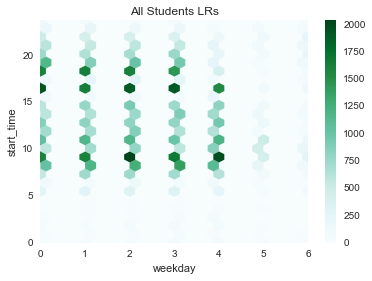
\includegraphics[scale=0.4]{img/all_students_lr_hexbin.png}\fixedlabel{all_students_lr_hexbin}{1a}
    & 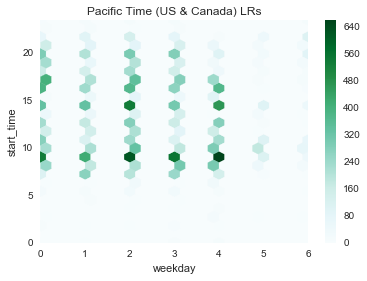
\includegraphics[scale=0.4]{img/pacific_lr_hexbin.png}\fixedlabel{pacific_lr_hexbin}{1b} \\
    2 & 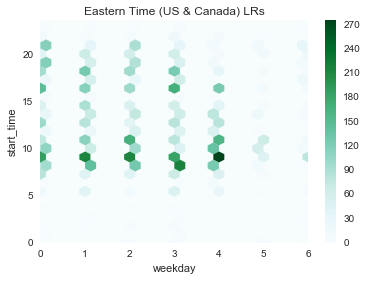
\includegraphics[scale=0.4]{img/eastern_lr_hexbin.png}\fixedlabel{eastern_lr_hexbin}{2a}
    & 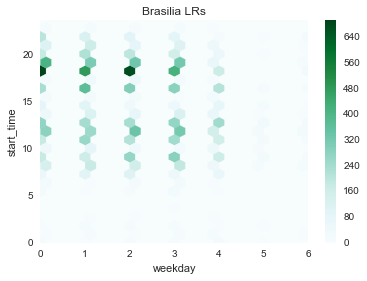
\includegraphics[scale=0.4]{img/brasilia_lr_hexbin.png}\fixedlabel{brasilia_lr_hexbin}{2b} \\
    3 & 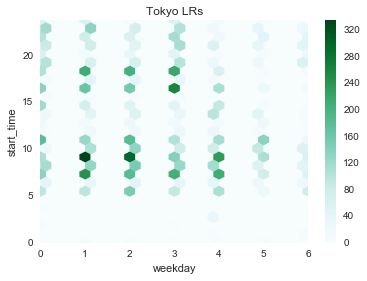
\includegraphics[scale=0.4]{img/tokyo_lr_hexbin.png}\fixedlabel{tokyo_lr_hexbin}{3a}
    & 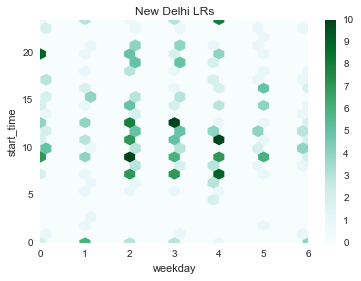
\includegraphics[scale=0.4]{img/new_delhi_lr_hexbin.png}\fixedlabel{new_delhi_lr_hexbin}{3b} \\
  \end{tabular}
  \caption{Weekly LR Densities by Timezone (weekday 0 = Monday)}
  \label{figtab:lr_densities_tz}
\end{table}

We see densities of lesson requests (LRs) in the span of the week as a function of
timezone (Table \ref{figtab:lr_densities_tz}). We learn a couple of things from
this visualization: 1) In general, most lessons start between 6 AM to 10 PM on
the weekdays, and 2) timezone might be a good predictor of when people will
take lessons. For example, compare Figures and \ref{pacific_lr_hexbin}
\ref{brasilia_lr_hexbin} in Table \ref{figtab:lr_densities_tz} -- people taking
lessons with Brasilia timezones tend to have most of their lessons happening
around 7 PM, but those on Time tend to have most of their lessons at 9 AM and 3
PM. Also, by the same token, Fridays are not as popular with people on Brasilia
timezones than people on Pacific Time.

\subsection{Algorithms and Techniques}

Given that we know how many people will be taking lessons, what their lesson
frequency is going to be for the month, and what their timezones are, my
algorithm would output a projected number of lessons in each weekly schedule
bucket (e.g. 0-4 local time, 4-8 local time, etc.).

The algorithm is quite effective for how simple it is: for all the lessons that
ever happened in the training data, put them all in a weekly schedule, and
directly compute the probabilities that lessons would be requested for each bin
(e.g. 0-4 local time, 4-8 local time, etc.). Then, for each business forecast,
we filter the training data to only give us "relevant" information. For
example, if we think that timezone is relevant, then for each business
forecast, we bring up data from that timezone, and we calculate the probability
that someone will take lessons during each of the schedule bins.  We then
multiply that probability distribution by the number of students and the lesson
frequency. We keep a tally of all the sums.

For instance, let's say we get a business forecast that has 10 students, 2
lessons a week, from Eastern (US \& Canada) time, and the training data shows
that the probability of a lesson request happening for each bin, is as follows:
$[0.1, 0.3, 0.1, 0.2, 0.3, 0.1]$. We multiply that by the number of students
and by the number of lessons per week.  Therefore, we get $[0.1, 0.3, 0.1, 0.2,
0.3, 0.1] \times 10 \times 2 = [2,6,2,4,5,2]$ respectively.

To be more precise, however, we actually smooth out the probabilities by adding
a uniform distribution of small values. So from our example, let's say a
timezone has a distribution $S$ and we add uniform distribution $U$:

\begin{equation}
\frac{
    \begin{array}[b]{r}
      \left S = [ 0.10, 0.30, 0.10, 0.20, 0.30, 0.10 ]\\
      + \left U = [ 0.01,0.01,0.01,0.01,0.01,0.01]
    \end{array}
  }{
  \left S + U = [0.11, 0.31, 0.11, 0.21, 0.31, 0.11 \right.]
  }
\end{equation}

We normalize it so that the sum is 1:

\begin{align}
\frac{
    \begin{array}[b]{r}
      \left S+U
    \end{array}
  }{
\left \sum{(S + U)} \right.
} &= \frac{
    \begin{array}[b]{r}
      \left [0.11, 0.31, 0.11, 0.21, 0.31, 0.11 \right.] \\
    \end{array}
  }{
\left 1.16 \right.
}\\
&= [0.095, 0.267, 0.095, 0.181, 0.267, 0.095]
\end{align}

Then we multiply the normalized sum by the number of lessons from the forecast. So if there's 10 lessons projected for the timezone of interest, we multiply by 10:

\begin{equation}
\begin{split}
  10 \times [0.095, 0.267, 0.095, 0.181, 0.267, 0.095] \\
  = [0.95, 2.67, 0.95, 1.81, 2.67, 0.95]
\end{split}
\end{equation}

Hence we expect about 1 lesson to happen for 0-4 local time, 2-3 lessons during
4-8 local time, etc.

The main point of adding the smoother (i.e. $[0.1, .... , 0.1]$) is to distrust
the observed probabilities. For example, just because in our lifetime, we've
observed that the sun rises every single day means that the probability that
the sun will rise again is $100\%$ \cite{additive_smoothing}. We cannot be
fully certain, so we think it's more like 99.99\% (close to $100\%$ but not
$100\%$). Similarly, suppose we've observed that for a certain timezone with
only a few lessons that no lessons ever happened from 0-4 AM -- it does not
mean that the probability that a lesson will happen in the range of 0-4 AM is
0. Smoothing out the observed probabilities would probably smooth out our
incomplete observations to match true probabilities. Another big benefit is
avoiding division by zero.  Encountering a new timezone, without the smoother,
by definition, would mean that observed probabilities would be 0. We avoid this
error by simply making use of the smoother.

The advantage of this algorithm is its simplicity, speed, and interpretability.
It is very simple and easy to understand, and its' predictions are quite fast,
Also, its error is quite small in comparison to the benchmarks, which makes it
a good candidate for the problem it is trying to solve.

\subsection{Benchmark}

For benchmarking purposes, I created two other models that were based on two
hypotheses. First, I made a model that assumes that schedules are distributed
equally (\emph{DumbModel}, Table \ref{tab:dumb}). Since we know from
visualizations that wee hours of the morning are clearly not as likely as the
other parts of the day (we also know that weekends are clearly not as popular
as weekdays), we expect this model to perform poorly. It is a good to include
as a benchmark, because we expect that our more complicated model should be
leaps and bounds better than this.  Second, I created a model that assumes
schedules are equally distributed in the range of hours when most people are
active (\emph{SmartModel}, Table \ref{tab:smarter}). We expect that
\emph{SmartModel} would be better than the dumb model, but we expect that our
model to beat the other two by a significant margin due to the fact scheduling
is not randomly distributed by any means.

\begin{table}[]
  \centering
  \caption{Dumb Model: Assumes lesson requests (naively) start randomly anytime}
  \label{tab:dumb}
  \begin{tabular}{|P{1cm}|P{1cm}|P{1cm}|P{1cm}|P{1cm}|P{1cm}|P{1cm}|P{1cm}|}
    \hline
                  & \textbf{Mon} & \textbf{Tue} & \textbf{Wed} & \textbf{Thu} & \textbf{Fri} & \textbf{Sat} & \textbf{Sun} \\
    \hline
    \textbf{0:00} & \Checkmark &\Checkmark &\Checkmark &\Checkmark &\Checkmark &\Checkmark &\Checkmark \\
    \textbf{0:15} & \Checkmark &\Checkmark &\Checkmark &\Checkmark &\Checkmark &\Checkmark &\Checkmark \\
    \textbf{0:30} & \Checkmark &\Checkmark &\Checkmark &\Checkmark &\Checkmark &\Checkmark &\Checkmark \\
    \textbf{.}    & \Checkmark &\Checkmark &\Checkmark &\Checkmark &\Checkmark &\Checkmark &\Checkmark \\
    \textbf{.}    & \Checkmark &\Checkmark &\Checkmark &\Checkmark &\Checkmark &\Checkmark &\Checkmark \\
    \textbf{.}    & \Checkmark &\Checkmark &\Checkmark &\Checkmark &\Checkmark &\Checkmark &\Checkmark \\
    \textbf{23:30} & \Checkmark &\Checkmark &\Checkmark &\Checkmark &\Checkmark &\Checkmark &\Checkmark \\
    \textbf{23:45} & \Checkmark &\Checkmark &\Checkmark &\Checkmark &\Checkmark &\Checkmark &\Checkmark \\
    \hline
  \end{tabular}
\end{table}

\begin{table}[]
  \centering
  \caption{Smart Model: Assumes lesson requests only start when people are generally awake}
  \label{tab:smarter}
  \begin{tabular}{|P{1cm}|P{1cm}|P{1cm}|P{1cm}|P{1cm}|P{1cm}|P{1cm}|P{1cm}|}
    \hline
                  & \textbf{Mon} & \textbf{Tue} & \textbf{Wed} & \textbf{Thu} & \textbf{Fri} & \textbf{Sat} & \textbf{Sun} \\
    \hline
    \textbf{.}    &. &. &. &. &. &. &.\\
    \textbf{.}    &. &. &. &. &. &. &.\\
    \textbf{.}    &. &. &. &. &. &. &.\\
    \textbf{6:00} & \Checkmark &\Checkmark &\Checkmark &\Checkmark &\Checkmark &\Checkmark &\Checkmark \\
    \textbf{6:15} & \Checkmark &\Checkmark &\Checkmark &\Checkmark &\Checkmark &\Checkmark &\Checkmark \\
    \textbf{.}    & \Checkmark &\Checkmark &\Checkmark &\Checkmark &\Checkmark &\Checkmark &\Checkmark \\
    \textbf{.}    & \Checkmark &\Checkmark &\Checkmark &\Checkmark &\Checkmark &\Checkmark &\Checkmark \\
    \textbf{.}    & \Checkmark &\Checkmark &\Checkmark &\Checkmark &\Checkmark &\Checkmark &\Checkmark \\
    \textbf{23:30} & \Checkmark &\Checkmark &\Checkmark &\Checkmark &\Checkmark &\Checkmark &\Checkmark \\
    \textbf{23:45} & \Checkmark &\Checkmark &\Checkmark &\Checkmark &\Checkmark &\Checkmark &\Checkmark \\
    \hline
  \end{tabular}
\end{table}

\section{Methodology}
\subsection{Data Preprocessing}

\begin{table}[]
  \centering
  \caption{Frequency of LRs Missing Timezone Over Months}
  \label{tab:freq_lrs_missing_timezone_over_months}
  \begin{tabular}{lrr}
    \hline
    \textbf{year} & \textbf{month} & \textbf{frequency} \\
    \hline
      2014 &  2  &    1\\
           &  3  &  134\\
           &  4  &   84\\
           &  5  &   69\\
           &  6  &   72\\
           &  7  &   73\\
           &  8  &   40\\
           &  9  &   50\\
           &  10 &   37\\
           &  11 &   14\\
           &  12 &   11\\
      2015 &  1  &   12\\
           &  2  &    5\\
      2016 &  7  &    7\\
           &  8  &    6\\
    \hline
  \end{tabular}
\end{table}



In order to create training and test sets, some data preprocessing had to
occur. First was the removal of 615 lesson requests that had missing timezone
information (Table \ref{tab:freq_lrs_missing_timezone_over_months}). It was
done because we could gather no useful information about when students actually
took lessons relative to their timezone from that data (i.e. we don't have an
idea of what ``morning", ``afternoon", or ``evening" is to them, which renders
their data useless for prediction). This could possibly have introduced a bias
in the models created. For instance, consider the case where most of the 615
lesson requests happened during mornings. Since I removed the data, it's
possible that the models might underestimate the probability of lesson requests
happening in the mornings. However, I think it is not a big problem, since this
data integrity issue is much less likely to happen with newer data. Training
data used to make predictions, as designed, would only look at a specified last
few months, which, over time, would lessen the impact of the possibly-biased
2014 data. In essence, problematic 2014 data would be phased out from being the
training set as we keep making predictions in the future.

Once the problematic data was removed, I transformed raw lesson request data
into schedules. I took the first 16 lesson requests of each person and
discarded the rest (Table \ref{tab:example_1st_16_lesson_requests}). 16 was
arbitrary -- it could have been smaller. These 16 lesson requests were then
projected onto a weekly schedule. In the weekly schedule (Table
\ref{tab:weekly_schedule_first_16_lrs:intermediary}), I looked for the highest
frequency, which I then used to filter out ones that were less than or equal to
half of the highest frequency (i.e. "noise", see Table
\ref{tab:weekly_schedule_first_16_lrs:final}). People generally take lessons
during the same time over the week, especially when they have elected to take
lessons regularly in the next two months (which we call a "progress plan").
However, they might reschedule for a different time for a bunch of reasons
(e.g. an urgent meeting at work had to happen which blocked them from taking
lessons at their scheduled lesson time). Filtering these statistical
fluctuations made sense.

Then, I labeled each schedule as being type 1 if there was only one weekly
schedule lesson, 2 if there were two entries, etc. We classify the user
schedule as belonging to a certain month based on when the first lesson request
happened. Thus, User $1$ in our training/test data would be represented as data
in Tables \ref{tab:user_summary:part_1} and \ref{tab:user_summary:part_2}.

\begin{table}[]
  \centering
  \caption{Example First 16 Lesson Requests of a User}
  \label{tab:example_1st_16_lesson_requests}
  \begin{tabular}{lrr}
    \hline
     & \textbf{user\_id} & \textbf{lr\_start\_datetime} \\
    \hline
     1 & 1   & 2016-09-21 08:00:00-04:00 \\
     2 & 1   & 2016-09-23 09:00:00-04:00 \\
     3 & 1   & 2016-09-26 09:00:00-04:00 \\
     . & .   & . \\
     . & .   & . \\
     . & .   & . \\
     14 & 1   & 2016-09-26 08:30:00-04:00 \\
     15 & 1   & 2016-09-26 09:00:00-04:00 \\
     16 & 1   & 2016-09-26 09:00:00-04:00 \\
    \hline
  \end{tabular}
\end{table}

\begin{table}[]
  \centering
  \caption{Weekly Schedule of a User: Intermediary Step}
  \begin{tabular}{|P{1cm}|P{1cm}|P{1cm}|P{1cm}|P{1cm}|P{1cm}|P{1cm}|P{1cm}|}
    \hline
                  & \textbf{Mon} & \textbf{Tue} & \textbf{Wed} & \textbf{Thu} & \textbf{Fri} & \textbf{Sat} & \textbf{Sun} \\
    \textbf{8:00} &  2 & & & & & & \\
    \textbf{8:15} &  & & & & & & \\
    \textbf{8:30} &  4 & & & & & & \\
    \textbf{8:45} &  & & & & & &\\
    \textbf{9:00} &  & & 5& &5& &\\
    \hline
  \end{tabular}
  \label{tab:weekly_schedule_first_16_lrs:intermediary}
\end{table}


\begin{table}[]
  \centering
  \caption{Weekly Schedule of a User: Final Step}
  \begin{tabular}{|P{1cm}|P{1cm}|P{1cm}|P{1cm}|P{1cm}|P{1cm}|P{1cm}|P{1cm}|}
    \hline
                  & \textbf{Mon} & \textbf{Tue} & \textbf{Wed} & \textbf{Thu} & \textbf{Fri} & \textbf{Sat} & \textbf{Sun} \\
    \textbf{8:00} &  & & & & & & \\
    \textbf{8:15} &  & & & & & & \\
    \textbf{8:30} &  \Checkmark & & & & & & \\
    \textbf{8:45} &  & & & & & &\\
    \textbf{9:00} &  & & \Checkmark& &\Checkmark& &\\
    \hline
  \end{tabular}
  \label{tab:weekly_schedule_first_16_lrs:final}
\end{table}

\begin{table}[]
  \centering
  \caption{Example User Summary: Part I}
  \label{tab:user_summary:part_1}
  \begin{tabular}{rrrrrrr}
    \textbf{user\_id} & \textbf{l1\_day} & \textbf{l1\_time} & \textbf{l2\_day} & \textbf{l2\_time} & \textbf{l3\_day} &\textbf{l3\_time} \\
    \hline
    1 & 0 & 8.5 & 2 & 9.0 & 4 & 9.0 \\
    \hline
  \end{tabular}
\end{table}

\begin{table}[]
  \centering
  \caption{Example User Summary: Part II}
  \label{tab:user_summary:part_2}
  \begin{tabular}{rrrrrrr}
    \textbf{start\_month} & \textbf{start\_year} & \textbf{schedule\_type}\\
    \hline
    9 & 2016 & 3\\
    \hline
  \end{tabular}
\end{table}




\subsection{Implementation}

\subsubsection{Code}

\emph{Scheduling Patterns.ipynb} is an iPython Notebook that goes opens the
anonymized lesson request data
(\emph{data/export\_lesson\_requests\_2016\_09\_08.pkl}) and aggregates them
into schedules for each user (\emph{unique\_user\_summaries.pkl}). The
predictions of different models over months of test data is done through
\emph{code/main.py}, which uses \emph{unique\_user\_summaries.pkl} to generate
the predictions (\emph{x\_model\_errors.pkl}). Sensitivity analysis is done
through \emph{code/sensitivity\_analysis.py}. Graphs of errors and the
accompanying tables were then generated through \emph{Predictions.ipynb}, which
makes use of \emph{x\_model\_errors.pkl}.

Models used in this experiment are located in \emph{code/models.py}. Each of
the models implement \emph{fit} and \emph{predict}. \emph{fit} takes in
training data as input and \emph{predict} takes in the business forecast, which
is a list of actual properties of the month-to-be-predicted (e.g. 20 requests
of 2x/week from Pacific Time, 10 requests of 1x/week from Eastern Time, etc.).

To calculate probabilities, weekly schedules (training and test data) were
internally represented by \emph{Schedule} and \emph{ActualSchedule} classes
(see \emph{code/schedule.py}). Each of those classes internally use a Pandas
\emph{DataFrame} -- rows are start times (0 to 23.75, inclusive), and columns
are days of the week (0 to 6, inclusive). All the models that have \emph{Prob}
in the name make use of \emph{Schedule} and \emph{ActualSchedule} for this
reason.

The class that is responsible for testing a model is \emph{BackTest}
(\emph{code/backtest.py}). It is responsible for splitting the processed data
into training and test sets.  \emph{BackTestMultiple} (also in
\emph{code/backtest.py}), is responsible for testing multiple models and builds
upon the former.

For more details, please take a look at the \emph{spec} folder. It has a bunch
of tests that describe how each of the classes are supposed to behave.


\subsubsection{Challenges}

One issue was using company name as a predictor variable/feature.  I was hoping
to examine whether or not knowing about a company could help us more accurately
predict when that person will take lessons.  Perhaps some companies are more
likely to take lessons during the morning than the evening as a function of
work culture and positions (e.g. a tech company with mostly tech employees
might have more flexibility as to when they take lessons than non-tech
companies with non-tech employees).

I tried to use it as a variable, however users are not associated with only one
company in the system, so we are left with the problem of figuring out which
company to assign to the user, which is difficult. Not solving for this problem
would mean that in joining the \emph{lesson request} and \emph{company} SQL
tables, lesson requests would be duplicated for users that are associated to
more than one company, which would skew the results. Their lesson requests
would have more representation than others' lesson requests, which might bias
the model towards over-predicting lesson requests for those times which have
lots of duplication and under-predicting lesson requests for the rest.

For example, consider company A and company B. Let's say company A is
``Twitter'' and B is ``TwitterGlobal". Basing on the naming convention, company
A seems like it is going to be a subset of B (Figure
\ref{fig:venn_a_subset_b}), but that does not seem to be the case -- they both
have elements that are not present in the other (Figure
\ref{fig:venn_a_and_b}).  What do we do with the people that they have in
common? Do we just label them A? Or should they be B? Or do we label them as
something else?

However, in terms of having a robust model that is able to generalize well
given new data, using company information might not be that useful. Everytime
we encounter a new company, by definition, we would have little to no data. In
those cases, we cannot make good predictions on company information alone.

Another issue was using legacy code as benchmark. There exists code that helps
predict student demand. I would have loved to use the code to see how it
performs against my model. However, code for it is not maintained and is hard
to understand, and the engineer who wrote it is no longer with us. That part of
the codebase will probably be deprecated in favor of this, which actually is
well-tested and heavily documented. Comparing the performance of the models
here with that black-box benchmark might give us more insight as to possible
weaknesses of my model, but due to the perceived return of investment, it was
not done at the time of this writing.

\begin{figure}[h!]
\centering
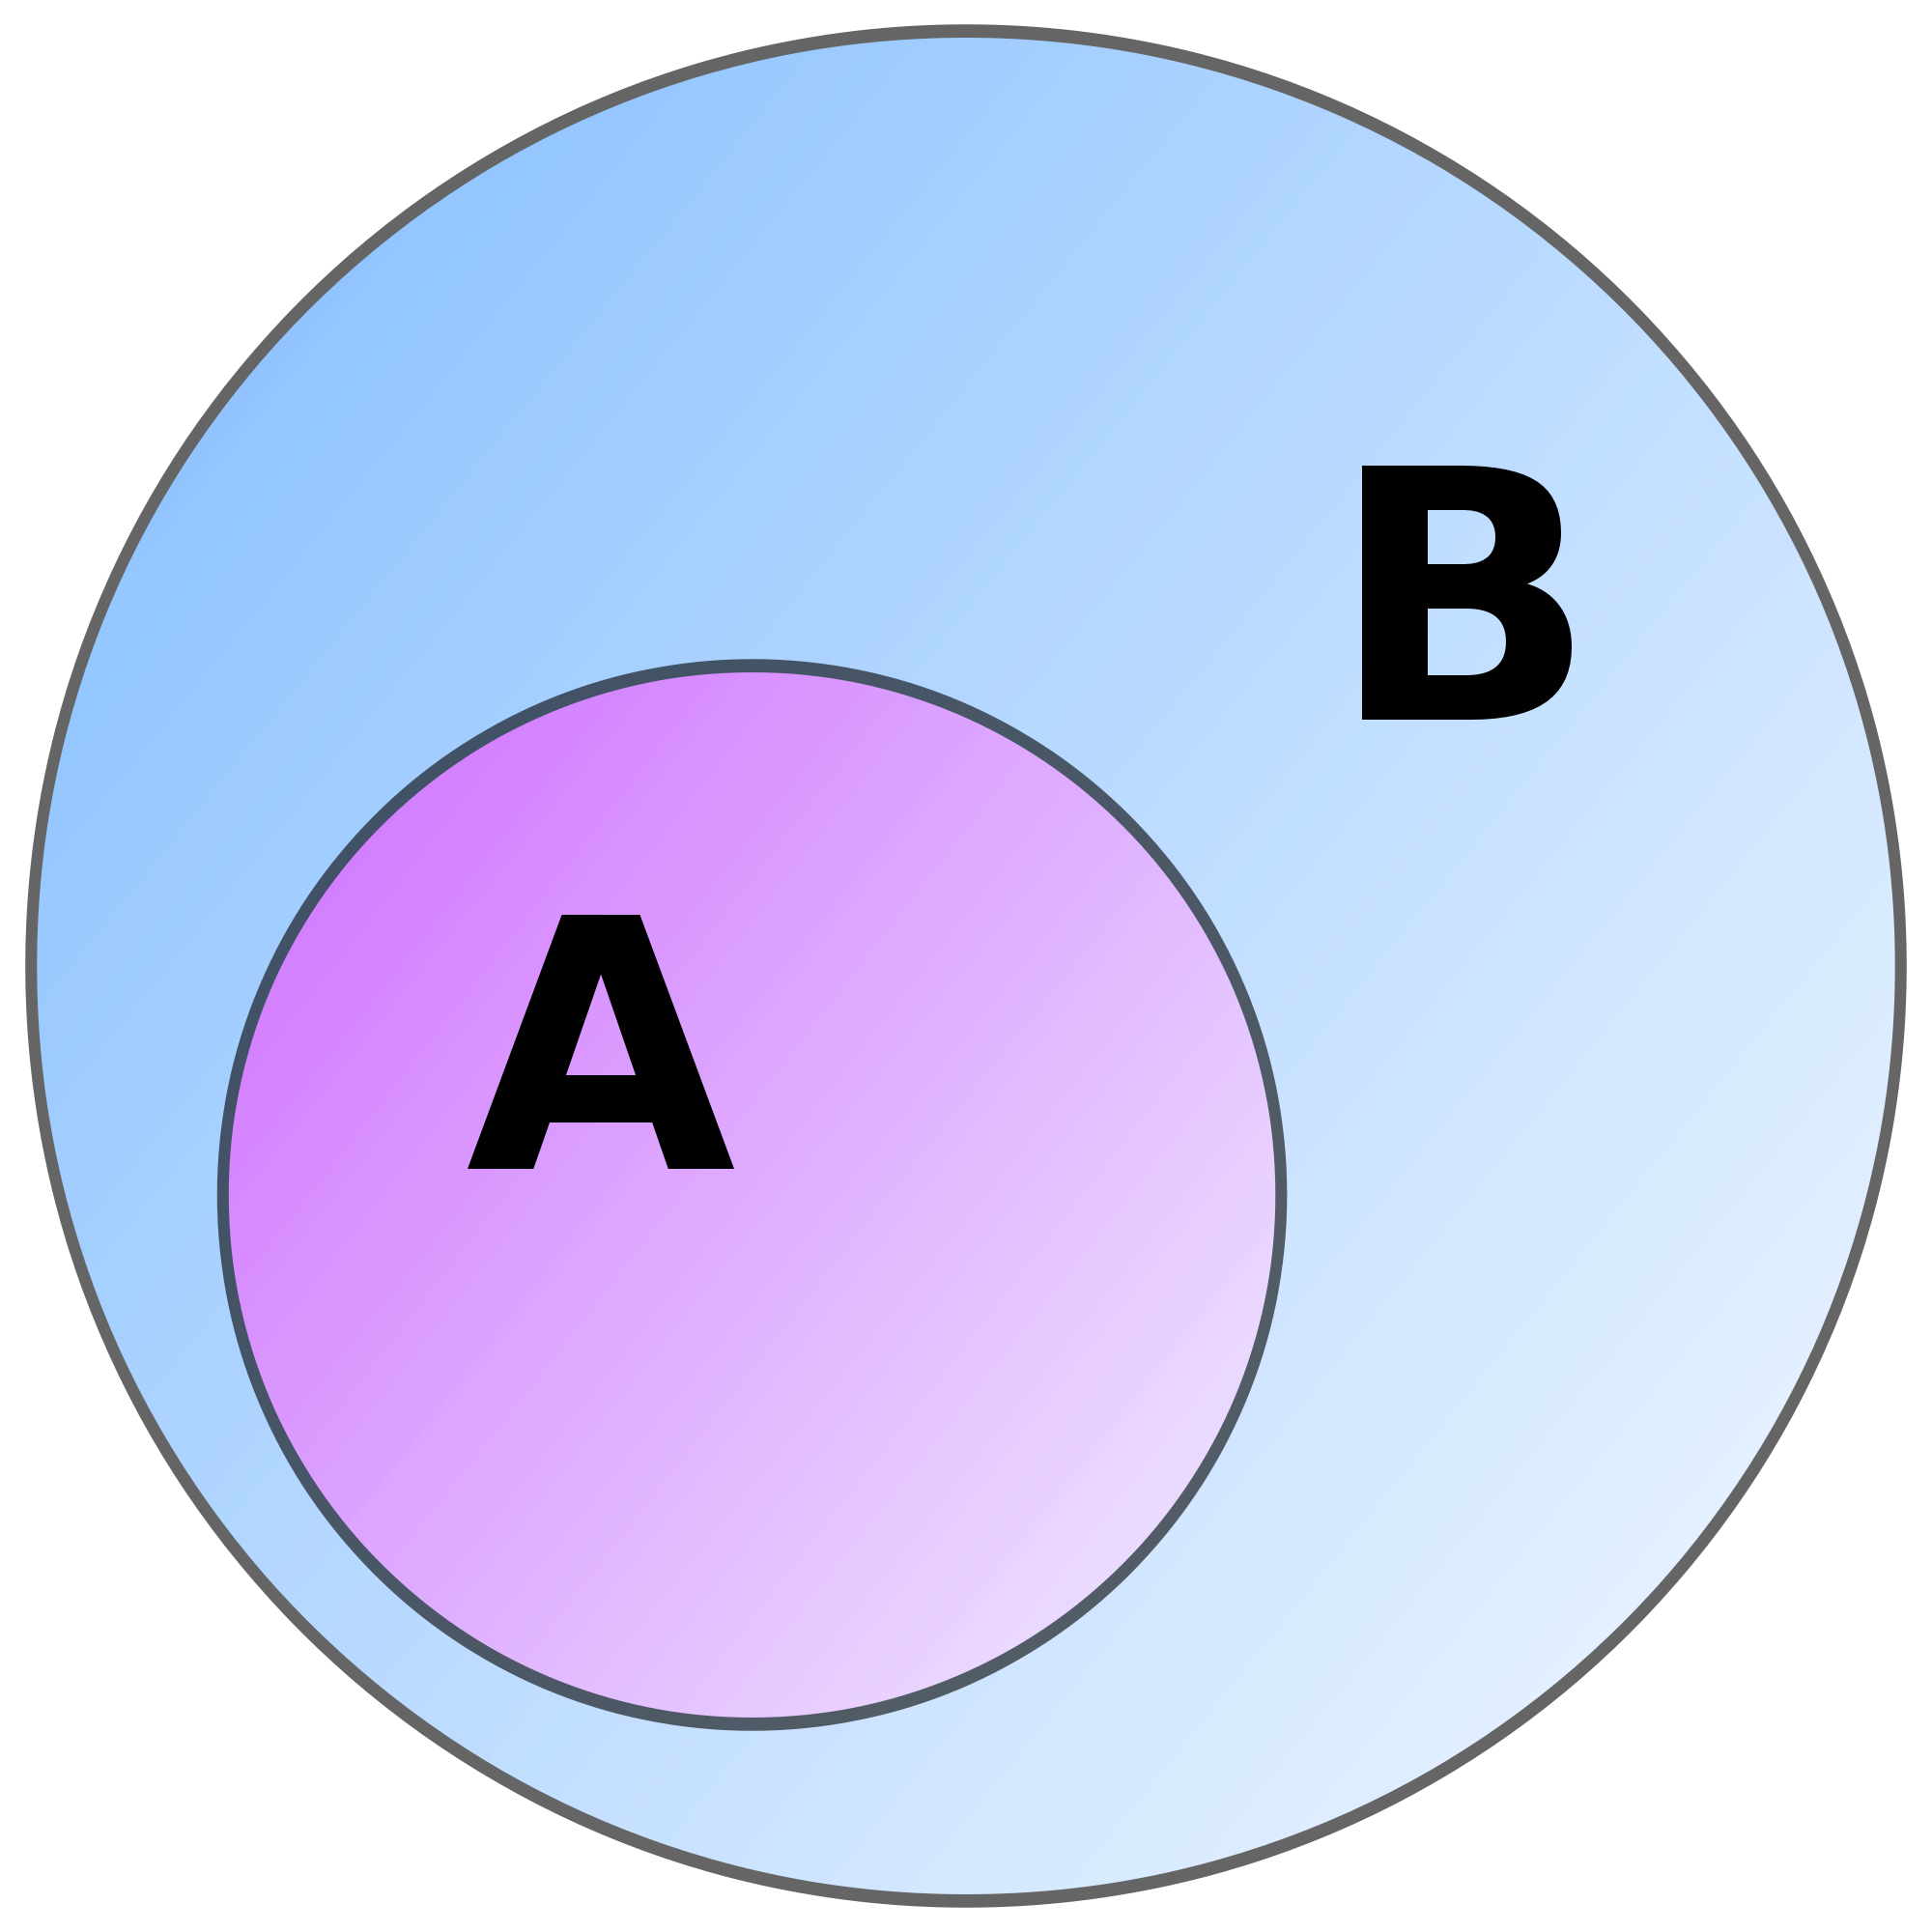
\includegraphics[scale=0.05]{img/venn_a_subset_b.png}
\caption{Company A is a subset of Company B}
\label{fig:venn_a_subset_b}
\end{figure}

\begin{figure}[h!]
\centering
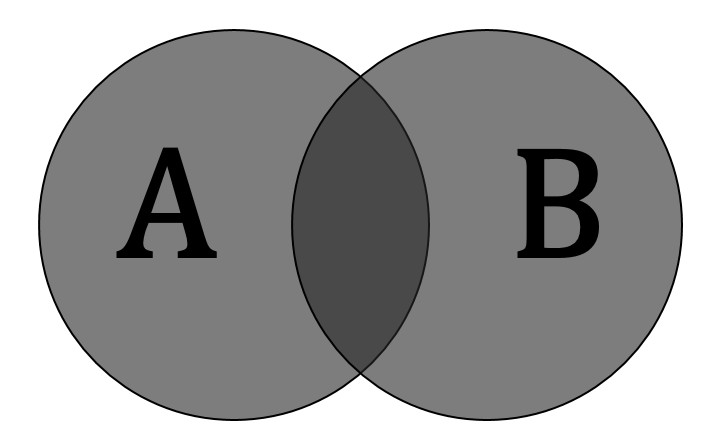
\includegraphics[scale=0.1]{img/venn_a_and_b.jpg}
\caption{Company A is not a subset of Company B}
\label{fig:venn_a_and_b}
\end{figure}

\subsection{Refinement}

Several ways were attempted to improve the performance of the algorithm.
First, I performed feature selection and created submodels: timezone only
(\emph{TimezoneProbModel}), lesson frequency only (\emph{LFProbModel}), lesson
frequency and timezone (\emph{LFTProbModel}). It turned out that
\emph{user\_tz} was the best predictor out of the two variables over several
months. Using lesson frequency by itself, and using lesson frequency in
combination with timezone resulted in a slightly less performant model.
\emph{GeneralProbModel}, which does not take into account either variables when
fine-tuning its training data, was also created. It performs slightly worse
than \emph{TimezoneProbModel}, but better than the other models. I was quite
convinced with using \emph{TimezoneProbModel} as the final model, but thanks to
sensitivity analysis (discussed at the Results section), I discovered a flaw.
It was mitigated by generating a meta model that makes use of both
\emph{TimezoneProbModel} and \emph{GeneralProbModel} predictions. More of this
is discussed below.

\section{Results}

\subsection {Model Evaluation and Validation}

\begin{table}[]
  \centering
  \caption{Average Mean Absolute Errors (11 months)}
  \label{tab:avg_mae_of_models}
  \begin{tabular}{rr}
    \textbf{model} & \textbf{average MAE over 12 months} \\
    \hline
    TimezoneProbModel &            6.467433 \\
    InterpolatedProbModel &        6.607820 \\
    GeneralProbModel &             6.893402 \\
    LFProbModel &                  7.023239 \\
    LFTProbModel &                 7.887060 \\
    SmartHeuristicModel &         12.062500 \\
    DumbModel &                   23.046296 \\
    \hline
  \end{tabular}
\end{table}

Over 11 months of test data (2015-09 to 2016-08), \emph{TimezoneProbModel}
performed the best (See Figure \ref{fig:mae_models} and Table
\ref{tab:avg_mae_of_models} for details; please note that only the benchmarks
and the best performing ones were kept to keep the graph from being cluttered).
It is not surprising -- looking at Table \ref{figtab:lr_densities_tz}, one
could see that timezone does carry information that helps us predict when a
student would take lessons. However, after doing sensitivity analysis, I
quickly learned that the model itself has a big weakness -- predicting
schedules of timezones it hasn't seen.

\begin{figure}[h!]
\centering
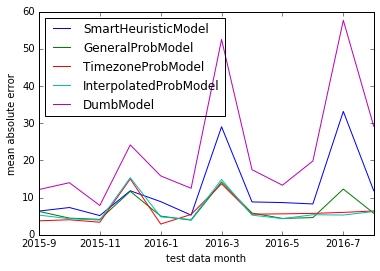
\includegraphics[scale=0.8]{img/mae_models.png}
\caption{Mean Absolute Errors over 12 months}
\label{fig:mae_models}
\end{figure}

Consider the scenario when a timezone we don't have much experience with (i.e.
sample size for the given timezone is very low). For example, at the time of
this writing, we only have one user schedule that has "Adelaide" as the
timezone. In my sensitivity analysis (\emph{code/sensitivity\_analysis.py}), I
created fake data to simulate predicting when lesson requests would happen from
an underrepresented timezone.  Specifically, I cloned data from one of the
previous months, labeled the clone as belonging to the under-represented
timezone (Adelaide).  I also then cloned the fake data (labeled as belonging to
Adelaide) for the next month after that. Again, the goal is to see how well
\emph{TimezoneProbModel} the robustness of the model. Not surprisingly, the
errors were huge -- by default, \emph{TimezoneProbModel} smooths out observed
probabilities, and when observed probabilities are zero (or close to zero),
smoothing them out will lead to a random 'flat' distribution, essentially
making a guess that even wee hours in the morning are as equally likely to have
lessons than other 'normal' times -- which we know is not the case.

To remedy this problem, I decided to create \emph{InterpolatedProbModel}, a new
model that interpolates between \emph{TimezoneProbModel} and
\emph{GeneralProbModel}. The latter assumes that it does not matter what
timezones people are coming from. When it gets a business forecast, it discards
timezone and uses information from all students' schedules -- not just
students' schedules that belong to the timezone of interest. It performs
slightly worse than \emph{TimezoneProbModel}, but it is still much better than
the two benchmarks, and it is able to handle underrepresented cases pretty
well. On fake unseen data I created, interpolation decreased error (compared to
\emph{TimezoneProbModel}) by about 89.6\% (from 172.88 to 17.95 MAE). After
cloning the unseen data again, \emph{InterpolatedProbModel} is able to take
advantage of \emph{TimezoneProbModel}'s more targeted approach (17.95 to 0.65
MAE), which shows the robustness and adaptability of the model (Table
\ref{tab:model_perf_underrepresented}).

\begin{table}[]
  \centering
  \caption{Model Performance on Underrepresented, Unseen Data}
  \label{tab:model_perf_underrepresented}
  \begin{tabular}{rrr}
    \textbf{model name} & \textbf{MAE on fake\_data\_1} & \textbf{MAE on fake\_data\_2} \\
    \hline
    GeneralProbModel & 13.319845 & 11.728293 \\
    InterpolatedProbModel & 17.947195 & 0.645111 \\
    TimezoneProbModel & 172.883495 & 0.676617 \\
    \hline
  \end{tabular}
\end{table}





The general idea of interpolation is the following.  When sample size for a
given timezone is small, weight the prediction of \emph{GeneralProbModel} more
heavily. When sample size is big enough, weight the prediction of
\emph{TimezoneProbModel} much more than \emph{GeneralProbModel}. If sample size
is not big enough, but not too small either, we weight the prediction of the
two models more equally.

Given the sample size of the timezone of interest, we pass that into a sigmoid
function to determine the weighting for each of the two models:

\begin{align}
  \text{TimezoneProbModel weight} = \frac{1}{1+e^{-\frac{x-80}{25}}}
\end{align}

where \emph{x} is the sample size of the given timezone of the business
forecast\cite{sigmoid_func}. This sigmoid function has the useful property of
outputting a weight between 0 and 1 (both inclusive). Figure
\ref{fig:sig_func_adjusted_for_interp} shows an example sigmoid function that
could be used for this problem:

\begin{figure}[h!]
\centering
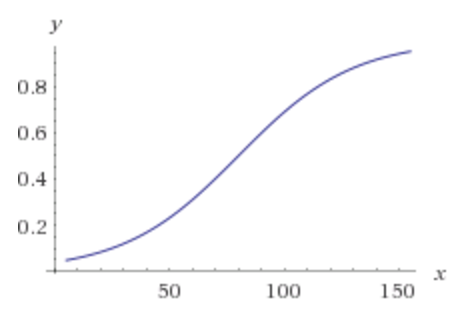
\includegraphics[scale=1]{img/special_sigmoid_func.png}
\caption{Sigmoid Function adjusted for interpolating between models}
\label{fig:sig_func_adjusted_for_interp}
\end{figure}

So when the lesson request sample size for the timezone of interest is close to
zero, \emph{TimezoneProbModel} is weighted weakly. However when the sample size
goes toward infinity, the weighting for \emph{TimezoneProbModel} approaches 1.
At the halfway point (i.e. where the timezone of interest has 80 lesson
requests in the training set), both \emph{TimezoneProbModel} and
\emph{GeneralProbModel} are weighted equally.  The parameters of the sigmoid
function were chosen by running an optimizer. In code, they are labeled
\emph{x\_offset} and \emph{x\_divisor}. \emph{x\_offset} directly affects where
the cut-off is, and \emph{x\_divisor} directly affects the smoothness of the
transition between two models. Values for \emph{x\_divisor} ranged from 1 to
50, while values for \emph{x\_offset} ranged from 100 to 150, depending on what
was in the training set.

Timezone carries information that could help predict when lessons will occur.
The caveat is when sample size is small -- we cannot trust the predictions of
\emph{TimezoneProbModel}. However, blending it with \emph{GeneralProbModel} via
\emph{InterpolatedProbModel} gives us the best of both worlds -- a model that
is robust and makes good predictions on under-represented data, yet it is also
a model that improves its predictions via the use of more relevant variables
once sample size increases.

\subsection{Justification}

In terms of average MAE, \emph{InterpolatedProbModel} presents a 71.3\%
improvement over \emph{DumbModel} and a 45.2\% improvement over
\emph{SmartHeuristicModel}, quite strong results compared to the two
benchmarks. As discussed before, interpolation decreased error (compared to
\emph{TimezoneProbModel}) by about 89.6\% on the example of unseen fake data
(Table \ref{tab:model_perf_underrepresented}), making it quite robust.

To get an intuitive sense of whether the \emph{InterpolatedProbModel} is
significant enough to have solved the problem, we could look at the predictions
on test data (Table \ref{tab:interpolated_bin_errors_over_months}). On this
table, the biggest errors (over- and under-estimates) were highlighted, and the
biggest of them all is about 30 lessons. Is being 30 lessons off a big problem?

In terms of hours, 30 lessons is equivalent to the following: 30 lessons
$\times$ 45 minutes per lesson $\times$ 1 hour per 60 minutes $ = 22.5$ hours.
On average, disregarding outliers, a task-based learning (TBL) teacher wants
20.79 hours per week (See Table \ref{tab:teacher_desired_hours} for teacher
desired hours). I think on average, one TBL teacher should be enough. I would
conservatively add 1 or 2 more teachers, just in case the lessons requested are
supposed to happen simultaneously (as opposed to being spread out).

How likely is this scenario? Given knowledge of how our predictions did on test
data, I'd say not very likely. There have been 66 bin predictions made ($11$
months $\times$ 6 bins per month). Five of those bins were off by at least 15
lessons. Thus, I claim that the probability of being off by at least 15 lessons
is about $5/66 = 9.09\%$, which is quite low. I would say that
\emph{InterpolatedProbModel} is a significant solution to the problem of
predicting student demand.

\begin{table}[]
  \caption{InterpolatedProbModel Bin Errors By Month}
  \centering
  \label{tab:interpolated_bin_errors_over_months}
  \begin{tabular}{lrrrrrrr}
    \toprule
    \textbf{time} & \textbf{0-4}& \textbf{4-8}& \textbf{8-12}& \textbf{12-16}& \textbf{16-20}& \textbf{20-24}&  \textbf{ss} \\
    \midrule
    \hline
    2015-9  &  -2.34 &   5.85 &   9.80 &  -7.31 &  -6.23 &   0.23 &        125.0 \\
    2015-10 &   1.38 &   2.81 & -11.80 &   1.21 &   1.33 &   5.07 &        120.0 \\
    2015-11 &  -0.18 &  -2.11 &  -7.45 &   6.61 &  -1.32 &   4.45 &         55.0 \\
    2015-12 &   3.88 &   0.41 & \textbf{-30.56} & \textbf{-17.63} &  \textbf{33.26} &  10.64 &        199.0 \\
    2016-1  &  -1.23 &   2.29 & -10.74 &  -1.65 &   5.44 &   5.89 &        137.0 \\
    2016-2  &   2.30 &  -3.16 &   8.12 &   2.12 &  -3.95 &  -5.42 &        141.0 \\
    2016-3  &   4.02 &  \textbf {20.75 } & \textbf{-27.48 } &   8.47 &  12.10 & \textbf{-17.85} &        485.0 \\
    2016-4  &   1.49 &   5.10 &  -6.30 &  -5.05 &  -4.39 &   9.16 &        119.0 \\
    2016-5  &   1.47 &   5.14 & -10.65 &   0.89 &   5.89 &  -2.73 &        120.0 \\
    2016-6  &   1.25 &   4.08 &  11.51 &  -4.27 & -10.48 &  -2.08 &        173.0 \\
    2016-7  &  -0.86 &   9.87 &  -4.15 &  -1.34 &   6.79 & -10.32 &        548.0 \\
    2016-8  &  -2.69 &   4.44 &   5.90 & -10.91 &  -5.25 &   8.51 &        239.0 \\
    \hline
    \bottomrule
  \end{tabular}
\end{table}

\begin{table}[]
  \caption{Task-Based Learning Teacher Desired Hours}
  \centering
  \label{tab:teacher_desired_hours}
  \begin{tabular}{rrr}
    \toprule
    \textbf{desired hours} & \textbf{desired hours} & \textbf{desired hours} \\
    \midrule
    \hline
    -30 & 16 & 30 \\
    0   & 17 & 30 \\
    5   & 18 & 32 \\
    6   & 20 & 35 \\
    6   & 20 & 35 \\
    6   & 20 & 40 \\
    8   & 20 & 40 \\
    10  & 20 & 40 \\
    10  & 20 & 45 \\
    10  & 20 & 50 \\
    10  & 20 & NaN\\
    10  & 20 & NaN\\
    10  & 23 & NaN\\
    10  & 24 & NaN\\
    11  & 25 & NaN\\
    12  & 25 & NaN\\
    12  & 25 & NaN\\
    15  & 25 & NaN\\
    15  & 25 & NaN\\
    15  & 25 & NaN\\
    15  & 25 & NaN\\
    15  & 28 & NaN\\
    15  & 30 & NaN\\
    15  & 30 & NaN\\
    15  & 30 & NaN\\
    15  & 30 & NaN\\
    15  & 30\\
    15  & 30\\
    16  & 30\\
    16  & 30\\
    \hline
    \bottomrule
  \end{tabular}
\end{table}



\section{Conclusion}
\subsection{Free-Form Visualization}

The visualization I chose is the error surfaces of the different models:
\emph{InterpolatedProbModel}, \emph{TimezoneProbModel},
\emph{GeneralProbModel}, \emph{LFProbModel}, and the two benchmarks
\emph{SmartHeuristicModel} and \emph{DumbModel} (See Table
\ref{figtab:error_surfaces}). Pay attention to the contour maps -- sections of
the surface that are close to zero are marked gray; ones that overestimate are
orange/red, but ones that underestimate are light blue/dark blue. A good model
in general would have less blue and orange areas.

Out of all the options shown, \emph{InterpolatedProbModel} seems to have the
least amount of blue/orange areas, so it's predictions in general are more spot
on than other models. \emph{GeneralProbModel}, for example, has a bunch more
orange spots, which means that it's overestimating more on average a bunch of
sections than \emph{InterpolatedProbModel}.

We could also see that the chosen model, \emph{InterpolatedProbModel}, is much
better (smoother) than the benchmarks\emph{SmartHeuristicModel} and
\emph{DumbModel}, judging by the jagged shapes -- these stalactites are huge
signs of underestimation.

Another visualization that provides evidence of \emph{InterpolatedProbModel}
being a good model is the error bars (Table \ref{figtab:error_bars}). One can
see that the errors for each bin, on average, are quite close to zero,
specially when compared to the two benchmarks (\emph{SmartHeuristicModel} and
\emph{DumbModel}). On average, the two benchmarks tend to severely over- and
under-estimate unlike \emph{InterpolatedProbModel}. The errors also have a much
smaller standard deviation than the benchmarks.

\begin{table}[ht]
  \centering
  \begin{tabular}{c@{\quad}ccc}
    & a & b \\
    1 & 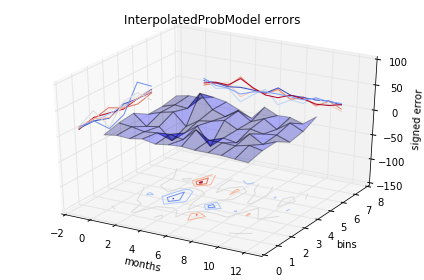
\includegraphics[scale=0.35]{img/error_surf_interpolated_prob_model.png}\fixedlabel{error_surf_interpolated_prob_model}{1a}
    & 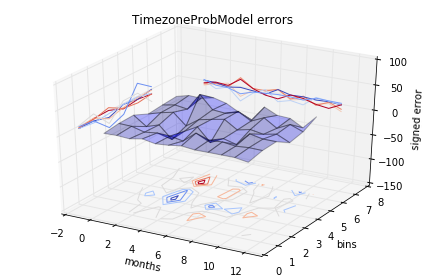
\includegraphics[scale=0.35]{img/error_surf_timezone_prob_model.png}\fixedlabel{error_surf_timezone_prob_model}{1b} \\
    2 & 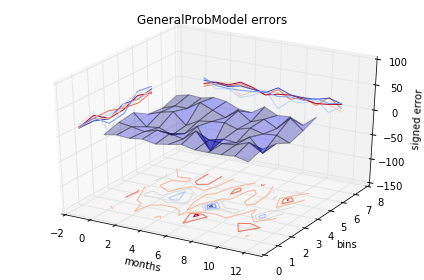
\includegraphics[scale=0.35]{img/error_surf_general_prob_model.png}\fixedlabel{error_surf_general_prob_model}{2a}
    & 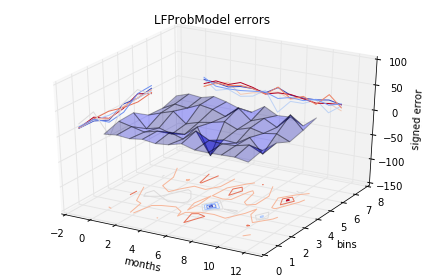
\includegraphics[scale=0.35]{img/error_surf_lf_prob_model.png}\fixedlabel{error_surf_lf_prob_model}{2b} \\
    3 & 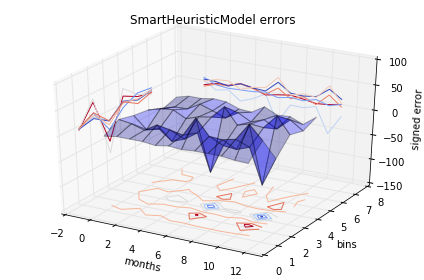
\includegraphics[scale=0.35]{img/error_surf_smart_heuristic_model.png}\fixedlabel{error_surf_smart_heuristic_model}{3a}
    & 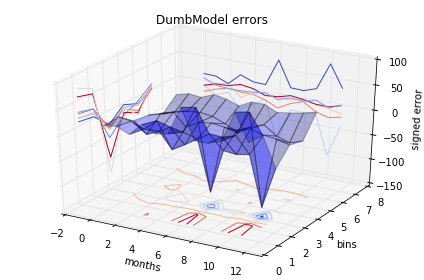
\includegraphics[scale=0.35]{img/error_surf_dumb_model.png}\fixedlabel{error_surf_dumb_model}{3b} \\
  \end{tabular}
  \caption{Error Surfaces of Different Models}
  \label{figtab:error_surfaces}
\end{table}

\begin{table}[ht]
  \centering
  \begin{tabular}{c@{\quad}ccc}
    & a & b \\
    1 & 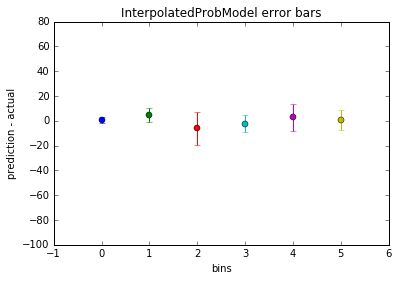
\includegraphics[scale=0.35]{img/error_bars_interpolated_prob_model.png}\fixedlabel{error_bars_interpolated_prob_model}{1a}
    & 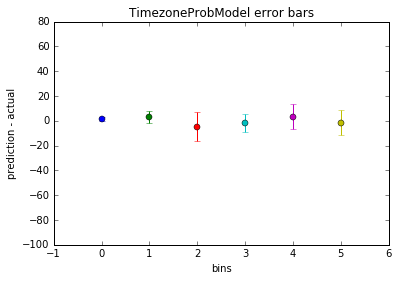
\includegraphics[scale=0.35]{img/error_bars_timezone_prob_model.png}\fixedlabel{error_bars_timezone_prob_model}{1b} \\
    2 & 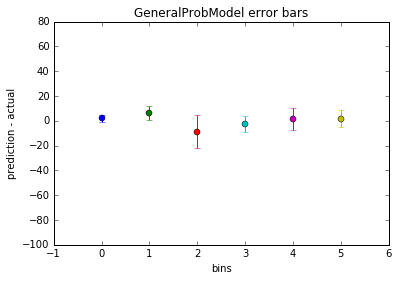
\includegraphics[scale=0.35]{img/error_bars_general_prob_model.png}\fixedlabel{error_bars_general_prob_model}{2a}
    & 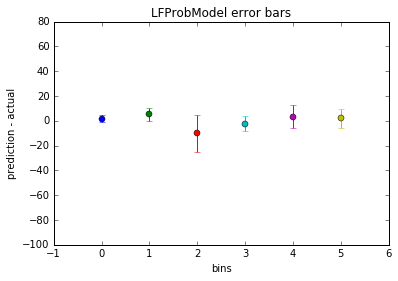
\includegraphics[scale=0.35]{img/error_bars_lf_prob_model.png}\fixedlabel{error_bars_lf_prob_model}{2b} \\
    3 & 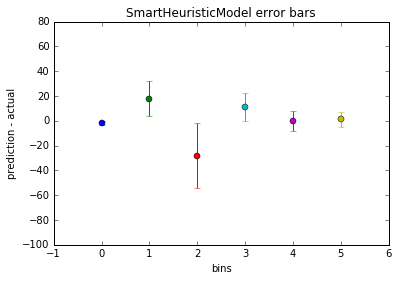
\includegraphics[scale=0.35]{img/error_bars_smart_heuristic_model.png}\fixedlabel{error_bars_smart_heuristic_model}{3a}
    & 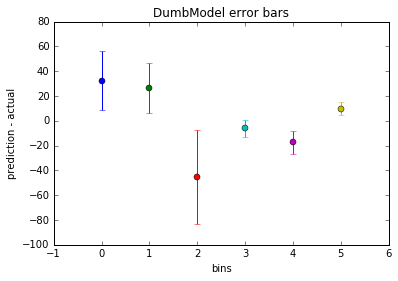
\includegraphics[scale=0.35]{img/error_bars_dumb_model.png}\fixedlabel{error_bars_dumb_model}{3b} \\
  \end{tabular}
  \caption{Error Bars of Different Models}
  \label{figtab:error_bars}
\end{table}

\subsection{Reflection}

In this project, I was able to create a model that predicts when students will
be taking lessons pretty well, given that we have information on their actual
lesson frequency and the timezones that they came from. The model is
essentially an ensemble of two submodels: \emph{GeneralProbModel} and
\emph{TimezoneProbModel}. When asked to predict when a student will be taking
lessons, the first makes a prediction without paying attention to the what the
timezone is. The training set consists of schedules without any care about
timezone, which has the benefit of being robust in predicting schedules of a
"new" timezone. On the other hand, the latter does make extensive use of
timezone when predicting when students will be taking lessons and generally
gets better results than the former -- it assumes that people in one timezone
might not be having the same scheduling patterns as others. The problem with
this approach, however, is when the model encounters unseen data (i.e. from a
"new" timezone). When the sample size is really low (e.g. 0), it's guess is
basically random, which we know performs poorly.  Thus, in this project, the
final model is one that interpolates between two models depending on sample
sizes of the different timezones based on the business forecast. This gives us
the best of both worlds.

One interesting thing I learned about this project is the Law of Diminishing
Returns. In the fitting step of \emph{InterpolatedProbModel}, I wanted to
figure out if there's an optimal cut-off point between the two models, and how
"soft" or "hard" the cut-off would be. To do so, the training data was
subdivided into two groups: sub-training and validation.  Sub-training data was
used to predict error on the validation set, which is the three most-recent
months in the training set. Then, I used an optimizer for a number of
iterations to find the best cut-off, which took several hours. What I optimized
for is the mean absolute error multiplied by the standard deviation of the
signed error of the bins. It improved the error-surface by a little bit (Table
\ref{figtab:error_surfaces}). Again, the error surface has more gray areas,
indicating that in a lot of predictions, the error is close to zero.  What I
found was that the cut-off ranged between about 100 and 150, and that it also
varied from "quite soft" to "hard", depending on what was in the validation
set.  However, it might not have been worth it, considering the amount of time
waiting for a result. \emph{InterpolatedProbModel} without optimizing for the
"cut-off" and "hardness" of the cut-off had about the same performance in terms
of MAE.

Overall, I am quite happy with the performance of \emph{InterpolatedProbModel}.
It will be used as part of a whole end-to-end system that would be used to
eventually predict when we need to hire teachers.

\subsection{Improvement}

This project, as described before, is supposed to be part of an end-to-end
system that would help forecast how many more teachers we need to hire in the
future. It would greatly be enhanced once the remaining parts of the system are
built, such as having an accurate model of what the business forecast would be
like (i.e. when business people say they think 50 students from Pacific
Timezone are going to join next month, we should also consider organic growth
(and churn) for that timezone and others). That would help create an accurate
business forecast, which would then be fed to the model to generate student
demand. Similarly, another thing that would improve this project is if the
student demand forecast is then connected with the recommender algorithm so we
could run simulations on when we think teachers would be needed next.


\bibliographystyle{plain}
\bibliography{references}

\end{document}
